% ----------------------------------------------- 
%  Plantilla LaTeX para el Trabajo Fin de Grado
%         Facultad de Ciencias
%        Universidad de Córdoba
%             Codificación utf8
%------------------------------------------------
%              Abril 2022
%------------------------------------------------


% MEJOR ABRIR DIRECTAMENTE EL DIRECTORIO PRINCIPAL DESDE EL VSCODE Y ASÍ LAS RUTINAS
% QUE TENGO PROGRAMADAS TE LAS DETECTA EL PROGRAMA

% A LA HORA DE COMPILAR HACERLO COMO SIEMPRE PARA PODER TENER EL PDF PRINCIPAL
% Y UNA VEZ HECHO ESO VIENDO QUE NO HAYA ERROR EN LA COMPILACIÓN DE ESE PDF 
% EJECUTAR EL ARCHIVO "compile.bat" QUE ESTÁ EN EL DIRECTORIO PRINCIPAL%
% LO QUE HACE ESE ARCHIVO ES GUARDAR UNA COPIA DEL PDF CON LA FECHA DE MODIFICACIÓN

% OTRA FORMA SI SE HA ABIERTO EL DIRECTORIO CON EN VSCODE ES USAR CONTROL+SHIFT+B


\documentclass[12pt,a4paper]{report}

% Fichero de estilo proporcionado
%%%%%%%%%%%%%%%%%%%%%%%%%%%%%%%%%%%%%%%%%%%%%%%%%%%%
%%
%% Este es el fichero 'estilo_TFG_CienciasUCO_2022.sty'
%%    con el estilo LaTeX para escribir los
%%          TRABAJOS FIN DE GRADO
%%                 de la 
%%          Facultad de Ciencias 
%%         Universidad de Córdoba
%               Abril 2022
%    
%           CODIFICAIÓN utf-8
%%%%%%%%%%%%%%%%%%%%%%%%%%%%%%%%%%%%%%%%%%%%%%%%%%%%%

% Hyperref
\usepackage[pdfa]{hyperref}
\hypersetup{
    colorlinks=true, %set true if you want colored links
    linktoc=all,     %set to all if you want both sections and subsections linked
    linkcolor=black,  %choose some color if you want links to stand out
    urlcolor=blue,
    citecolor=red,    % PDF metadata
    pdfauthor={José Estepa Ruiz},
    pdftitle={Trabajo Fin de Grado 2024-25},
    pdfsubject={TFG},
    pdfkeywords={DFT},
    pdfproducer={Latex with hyperref},
    pdfcreator={Visual Studio Code}
}

% Idioma castellano 
\usepackage[utf8]{inputenc}
\usepackage[T1]{fontenc}
\usepackage[spanish,es-tabla]{babel}

% AMS Packages
\usepackage{amsmath,amssymb,amsfonts,amsthm}
\usepackage[version=4]{mhchem}

% Other Packages
\usepackage{textcomp}
\usepackage{enumitem}
\usepackage{dsfont}
\usepackage[usenames]{color} %para usar colores con el comando \textcolor{nombre color en inglés}{texto}
\usepackage{framed}
\usepackage{xcolor}

% Tamaño de la página
\usepackage[left=2.5cm,right=2.5cm,top=2cm,bottom=2cm]{geometry}

\usepackage{setspace}
\linespread{1.3}
\setlength{\parindent}{1cm}
\usepackage{makeidx}
\newcommand*\emptyPage{\newpage\null\thispagestyle{empty}\newpage}
\decimalpoint    % Usa el punto como separador decimal

% Paquetes auxiliares  (incluir aquellos que se necesiten)
\usepackage[dvipsnames]{xcolor} % Para usar colores
\usepackage{tikz}                        % Para dibujar
\usepackage[strict]{changepage}          % Para redefinir márgenes en mitad del documento

% Para matemáticas
\usepackage{amsmath}
\usepackage{amsfonts}
\usepackage{amssymb}

% Para gráficos
\usepackage{graphicx}
\usepackage{subfigure}
\usepackage{float}
\usepackage{appendix}   % Contiene mandatos adicionales para apéndices
\usepackage{titlesec}   % Para redefinir capítulos, secciones,...
\usepackage{longtable}  % Para tablas grandes

% Para las cabeceras y pies (luego se redefine cuando haga falta)
\usepackage{fancyhdr}   % Para las cabeceras
\pagestyle{fancy} 
\fancyhf{}
\renewcommand{\headrulewidth}{0pt}
\renewcommand{\footrulewidth}{0pt}

% Para el fondo de la portada
\usepackage{eso-pic}
\newcommand\BackgroundPic{%
\put(0,0){%
\parbox[b][\paperheight]{\paperwidth}{%
\vfill
\centering
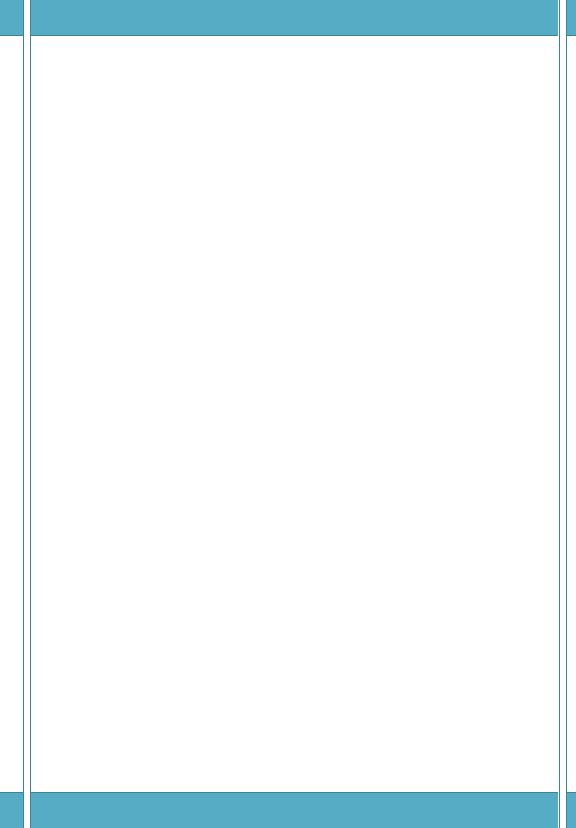
\includegraphics[width=\paperwidth,height=\paperheight,%
keepaspectratio]{img/fondo_portada.png}%
\vfill
}}}

% Estilo de capítulo, secciones...
\titlespacing*{\chapter}{0pt}{50pt}{40pt}
\titleformat{\chapter}[display]
  { \sffamily\bfseries\Large\color{blue}}
  {\filleft\MakeUppercase{\chaptertitlename}\ \Huge\sffamily{\arabic{chapter}}\ 
  }  
  {4ex}
  {\titlerule
   \vspace{2ex}%
   \filright}
  [\vspace{2ex}\hrule\vspace{2pt}%
   \titlerule]
   
\titleformat{\section}[hang]
  {\large \scshape\bfseries}
  {\color{blue}  \thesection .}
  {1ex}{\color{blue}}[\quad]
{}

\titleformat{\subsection}[runin]
  { \scshape\bfseries}
  {\color{blue}  \thesubsection .}
  {1ex}{\color{blue}}[\quad]
{}

%%%%%%%%%%%%%%%%%%%%%%%%%%%%%%%%%%%%
% Para los códigos 
\usepackage{listings}

% Para código Matlab
\lstset{language=Matlab,
  keywords={break,case,catch,continue,else,elseif,end,for,function,
      global,if,otherwise,persistent,return,switch,try,while,diary,
      clear,clc,who,whos,help,helpwin,linspace,length,ans,doc,floor,
      ceil,max,min,sum,prod,sort,round,sign,fix,mean,exp,sin,cos,tan,
      input,fprint,load,save,disp,fopen,fclose,inline,function,feval,
      global,return,poly,polyval,roots,solve,fzero, poly2sym,hold,plot,
      polyfit,ppval,spline,interp1,quad,quadl,quadgk,inv,\,lu,cond,spdisgs,
      magic,ode*,ode45,ode23,flops,rref,pinv,chol,zeros,ones,rand,sparse,
      tic,toc,diag,eye,speye,espones,spy,syms,diff,dsolve,simplify,ezplot},
   basicstyle=\small \ttfamily,
   keywordstyle=\color{blue},
   commentstyle=\color{webgreen},
   stringstyle=\color{webtinto},
   numbers=left,
   numberstyle=\tiny\color{gray},
   stepnumber=1,
   numbersep=10pt,
   backgroundcolor=\color{white},
   tabsize=4,
   showspaces=false,
   showstringspaces=false,
   frame=LtbR,
   framerule=0.5pt,
   aboveskip=0.5cm,
   framextopmargin=3pt,
   framexbottommargin=3pt,
   framesep=0pt,
   rulesep=.4pt,
   backgroundcolor=\color{gray96},
   rulesepcolor=\color{black}
}

% Para código ISE
\lstdefinelanguage{ISE} {
  morekeywords={library,use,entity,is,port,in,out,end,
               architecture,of,is,signal,begin,process,then,
               port,downto,if,and,then,else},
  sensitive=false,
  emph={STD_LOGIC_1164,
        STD_LOGIC_ARITH,
        STD_LOGIC_UNSIGNED,
        IEEE,
        ALL,
        STD_LOGIC,
        STD_LOGIC_VECTOR}, 
  emphstyle=\color{magenta},
  morecomment=[l]{--},
  basicstyle=\small \ttfamily,
  keywordstyle=\color{blue},
  commentstyle=\color{webgreen},
  stringstyle=\color{webtinto},
  numbers=left,
  numberstyle=\tiny\color{gray},
  stepnumber=1,
  numbersep=10pt,
  backgroundcolor=\color{white},
  tabsize=4,
  showspaces=false,
  showstringspaces=false,
  frame=LtbR,
  framerule=0.5pt,
  aboveskip=0.5cm,
  framextopmargin=3pt,
  framexbottommargin=3pt,
  framesep=0pt,
  rulesep=.4pt,
  backgroundcolor=\color{gray96},
  rulesepcolor=\color{black}
}

% Para generar índice con hipervínculos
\usepackage{hyperref}
\hypersetup{
    colorlinks,
    citecolor=webgreen,
    filecolor=black,
    linkcolor=webblue,
    urlcolor=webtinto,
}

% Colores definidos
\definecolor{azul}{rgb}{65,105,225}
\definecolor{webgreen}{rgb}{0,.5,0}
\definecolor{webgray}{rgb}{.753,.753,.753}
\definecolor{webblue}{rgb}{0,0,.8}
\definecolor{webtinto}{rgb}{0.73,0.00,0.00}
\definecolor{gray96}{gray}{.96}

% Algunas redefiniciones 
%\renewcommand{\contentsname}{Índice general}
%\renewcommand{\partname}{Parte}
%\renewcommand{\appendixname}{Apéndice}
%\renewcommand{\figurename}{Figura}
%\renewcommand{\listfigurename}{Índice de figuras}
%\renewcommand{\chaptername}{Capítulo}
%\renewcommand{\bibname}{Bibliografía}

\usepackage{graphicx}
\usepackage{subcaption}
\usepackage[labelfont=bf,labelsep=period,font={footnotesize,it}]{caption}
\usepackage{svg}
\usepackage{tikz}
\usepackage{calc}
\usepackage{booktabs}
\usepackage{xcolor}
\usepackage{float}
\usepackage{appendix}   % Contiene mandatos adicionales para apéndices
\usepackage{longtable}
\usepackage{physics}
\usepackage{upgreek} % para poner letras griegas sin cursiva
\usepackage{cancel} % para tachar
\usepackage{multirow}
\usepackage{lscape}
\usepackage{wrapfig}
\usepackage{multicol}
\usepackage{verbatim} % comentarios
\usepackage{pdfpages}
\usepackage{mathdots} % para el comando \iddots
\usepackage{mathrsfs} % para formato de letra
\usepackage{stackrel} % para el comando \stackbin

%% ENTORNO TEOREMA EN INGLES
\newtheorem{theorem}{Theorem}[section] %se usa \begin{theorem}[Nombre del teorema si lo tiene] Enunciado \end{theorem}
\newtheorem{lemma}[theorem]{Lemma}
\newtheorem{proposition}[theorem]{Proposition}
\newtheorem{corollary}[theorem]{Corollary}
\newtheorem{definition}[theorem]{Definition}
\newtheorem{example}[theorem]{Example}
\newtheorem{xca}[theorem]{Exercise}
\newtheorem{remark}[theorem]{Remark}
\renewcommand*{\proofname}{Proof} %para que escriba Demostración en lugar de proof; se usa \begin{proof} Prueba \end{proof}

\usepackage[nottoc]{tocbibind}

% BibTeX
\bibliographystyle{doc/nf}

% Useful personal commands
\newcommand{\centigrade}{$^{\circ}$}
\newcommand{\mum}{\mu\text{m}}
\newcommand{\muA}{\mu\text{A}}
\newcommand{\nA}{\text{nA}}

\newenvironment{dedication}
{
   \cleardoublepage
   \thispagestyle{empty}
   \vspace*{\stretch{1}}
   \hfill\begin{minipage}[t]{0.66\textwidth}
   \raggedright
}
{
   \end{minipage}
   \vspace*{\stretch{3}}
   \clearpage
}

\usepackage[spanish]{datetime}

%%%% Nuevas definiciones %%%%%%%%%%%%%%%%%%%%%%%%%%%%%%%

%--------------------------------------------------------------------------------------
% CAMBIAR LOS DATOS EN CADA CASO 

\newcommand{\titulacion}{Grado de Física}                  
                                                      
\newcommand{\titulo}{Método del Funcional de la Densidad para estructura electrónica de moléculas} % Título
\newcommand{\codigo}{FS24-031-FSC}      % Código
\newcommand{\tipo}{Trabajo teórico-práctico}            
% Trabajo teórico--práctico general
                                          		     % Trabajo de iniciación a la investigación
                                                      % Trabajo en empresa
                                                      % Idea de negocio
                                                      % Propuesta científico--técnica
                                                      % Trabajo docente
                                          
\newcommand{\autor}{José Estepa Ruiz}     % Autor
\newcommand{\fecha}{\today}                 % Fecha de entrega
%--------------------------------------------------------------------------------------
\newcommand{\nomfig}{Figura}                         
\newcommand{\nomfigs}{figuras} 

% Si se quiere que las figuras se denominen ilustraciones comentar las dos órdenes
% anteriores y descomentar las dos que siguen 

%\newcommand{\nomfig}{Ilustración}                         
%\newcommand{\nomfigs}{ilustraciones}   


%--------------------------------------------------------------------------------------

% Empieza el documento
\begin{document}




% No cambiar  %%%%%%%%%%%%%%%%%%%%%%%%%%%%%%%%%%%%%%%%%%%%%%%%%%%%%%%%%%%%
%%%%%%%%%%    NO CAMBIAR   %%%%%%%%%%%%%%%%%%%%%%%%%%%%%
% Inclusión automática de la portada, tribunal e índices
%%%%%%%%%%    NO CAMBIAR   %%%%%%%%%%%%%%%%%%%%%%%%%%%%%%

% PORTADA----------------------------------
\AddToShipoutPicture*{\BackgroundPic}
\begin{titlepage}
\begin{center}
\Large UNIVERSIDAD DE CÓRDOBA\\[0.5 cm]
\large  \textbf{Facultad de Ciencias}\\[1.25 cm]
\large \textbf{\titulacion}\\[1.25 cm]
\Large  Trabajo Fin de Grado\\[2.25 cm]
\Huge   \titulo
\end{center}
\vspace{1.25cm}
\noindent {\large Código del TFG: \textbf{\color{blue}\codigo}}\\[0.3cm]
\noindent {\large Tipo de TFG: \textbf{\color{blue}\tipo}}\\[0.5cm]
{\color{blue}\hrule}
\vspace{0.5cm}
\noindent \Large{Autor: \autor}
\vfill
\begin{center}
 
\includegraphics[width=6cm]{img/Logotipo_I_Facultad_de_Ciencias_Fondo_blanco_negativo.png} 
\end{center}
\vfill
\rightline{\fecha ~ \currenttime}
\end{titlepage}
\renewcommand{\baselinestretch}{0.9}
\ClearShipoutPicture

 %%%%%%%%%%%%%%%%%%%%%%%%%%%%%%%%%%%%%%%%%%%%%%%%%%%%%%%%%%%%%%%%%%




   % Dejar esta línea (incluirá el fichero portada.tex proporcionado, que no hay que modificar)
% Fin de No cambiar %%%%%%%%%%%%%%%%%%%%%%%%%%%%%%%%%%%%%%%%%%%%%%%%%%%%%%%

%%%% \fancypagestyle{plain}{
\fancyfoot[R]{\large{pág. \thepage}}
}

\pagestyle{fancy} 

\chapter*{Agradecimientos}

Incluir los agradecimientos, si procede. % Agradecimientos y/o dedicatoria si procede (si no comentar esta línea)

% No cambiar  %%%%%%%%%%%%%%%%%%%%%%%%%%%%%%%%%%%%%%%%%%%%%%%%%%%%%%%%%%%%
% INDICES-----------------------------------

% Genera el índice de contenidos------------

\fancypagestyle{plain}{
\fancyfoot[R]{\small pág. \thepage} 
}
\tableofcontents
\addcontentsline{toc}{chapter}{Índice general}

\renewcommand{\baselinestretch}{1.5}

% Genera el índice de figuras---------------
\fancypagestyle{plain}{
\fancyfoot[R]{\small pág. \thepage} 
}
\renewcommand{\listfigurename}{Índice de \nomfigs}
\renewcommand{\figurename}{\nomfig}

\listoffigures
\addcontentsline{toc}{chapter}{Índice de \nomfigs}


% Genera el índice de tablas---------------
\fancypagestyle{plain}{
\fancyfoot[R]{\small pág. \thepage}
}
\listoftables
\addcontentsline{toc}{chapter}{Índice de tablas}


% Para las cabeceras del resto

\pagestyle{fancy} 
\fancyhf{}
\fancyfoot[R]{\small pág. \thepage}
\renewcommand{\headrulewidth}{0pt}
\renewcommand{\footrulewidth}{0pt}  % Dejar esta línea (incluirá el fichero indices.tex proporcionado, que no hay que modificar)
% Fin de No cambiar %%%%%%%%%%%%%%%%%%%%%%%%%%%%%%%%%%%%%%%%%%%%%%%%%%%%%%%

%%% \chapter*{Resumen}
\addcontentsline{toc}{chapter}{Resumen. Palabras clave}

Escriba aquí un resumen de la memoria en castellano que contenga entre 100 y 300 palabras. Las palabras clave serán entre 3 y 6.

\paragraph{Palabras clave:} palabra clave 1; palabra clave 2; palabra clave 3; palabra clave 4 









\chapter*{Abstract}
\addcontentsline{toc}{chapter}{Abstract. Keywords}

Insert here the abstract of the report with an extension between 100 and 300 words. 

\paragraph{Keywords:} keyword1; keyword2; keyword3; keyword4
          % Resumen (insertar en el fichero resumen.tex proporcionado, el resumen en español e inglés)

%%%%%%%%%%%%%%%%%%%%%%%%%%%%%%%%%%%%%%%%%%%%%
%%%%%%%%%%%%%%%%%%%%%%%%%%%%%%%%%%%%%%%%%%%%% A PARTIR DE AQUÍ SE INCLUYEN LOS CAPÍTULOS
%%%%%%%%%%%%%%%%%%%%%%%%%%%%%%%%%%%%%%%%%%%%%

\chapter{TEORIA}

% \section{¿Qué es el DFT?}

\subsection{Definición}

\subsection{Problema con la ecuación de Schrödinger} 

Vamos a ponernos en la situación en la que nos gustaría describir las propiedades de una colección de átomos bien definidas, como podría ser un cristal o una molécula.

Una de las cosas fundamentales que nos gustaría conocer sobre esos átomos es su energía, y sobre todo como cambiaría ésta si movemos los átomos.

Tenemos que tener en cuenta que los núcleos son muchísimo más pesados que los electrones. De esta manera los electrones responden mucho más rápido a cambios en su entorno que los propios núcleos.

Para ello primero resolvemos las ecuaciones que describen el movimiento de los electrones, con posiciones fijas de los núcleos atómicos. Encontraremos el estado fundamental para un conjunto de electrones, de manera que por la aproximación de Born-Oppenheimer podemos considerar como problemas matemáticos distintos el de los electrones y el del núcleo.

Si tenemos $M$ núcleos en las posiciones $\va{R}_1 , \dots , \va{R}_M$, podemos expresar la energía fundamental del estado como función de la posición de estos núcleos: $E = E(\va{R}_1 , \dots , \va{R}_M)$. Conociendo esta energía como la energía potencial adiabática de la superficie de los átomos.

Por otra parte para los $N$ electrones que conforman el sistema, la ecuación a resolver es la de Schrödinger: 

\begin{equation}
    \left[ \frac{\hbar^2}{2m} \sum_{i=1}^{N} \laplacian_i + \sum_{i=1}^{N} V(\va{r}_i) + \sum_{i=1}^{N} \sum_{j<i} U(\va{r}_i , \va{r}_j) \right] \psi = E \psi
\end{equation}


Para el hamiltoniano que hemos elegido, $\psi$ es la función de onda electrónica que es función de las coordenadas espaciales de cada uno de los $N$ electrones, $\psi = \psi \left( \va{r}_{1} , \dots , \va{r}_{N} \right)$  y $E$ es la energía del estado fundamental de los electrones.

Debido a las propiedades de los electrones la función de onda la podemos poner como producto de cada una de las funciones de onda individuales de cada uno de los N electrones, $\psi = \psi_{1} \left( \va{r} \right) \cdots \psi_{N} \left( \va{r} \right)$ 

Es importante saber que $N \gg M$, ya que por cada núcleo hay varios electrones asociados. Esto nos da cuenta de que resolver la ecuación de Schrödinger para materiales prácticos es muy complicado por la cantidad de dimensiones y ecuaciones a resolver. 

La situación se complica aún más cuando miramos el hamiltoniano, siendo el término más crítico el de interacción entre electrones desde el punto de vista de resolver la ecuación. Para un electrón dado no es simple calcular $\psi_{i} \left( \va{r} \right)$ ya que depende del resto de electrones del sistema.

Una cosa que si que podemos medir de forma mas sencilla es la probabilidad de que los $N$ estén en una configuración particular de coordenadas $\va{r}_{1} , \dots , \va{r}_{N}$. De tal manera que una cantidad que está relacionada con esta probabilidad es la densidad de electrones en una determinada posición del espacio, 

\begin{equation}
    n(\va{r}) = 2 \sum_i \psi^*_i (\va{r}) \psi_i (\va{r})
\end{equation}

, expresión en la cual ya se tiene en cuenta el Principio de exclusión de Pauli con el 2 que precede a la suma.

Lo importante de esta discusión es que la densidad electrónica, $n(\va{r})$, es un parámetro del sistema que sí podemos medir físicamente y de la que podemos obtener gran parte de la información del sistema al estar relacionada con la función de onda total  $\psi = \psi \left( \va{r}_{1} , \dots , \va{r}_{N} \right)$.


 

% \subsection{Definición}

% \subsection{Problema con la ecuación de Schrödinger}

\section{Aproximación de Thomas-Fermi}

\section{Teoremas de Hoohenberg-Kohn}   

\section{Ecuaciones de Kohn-Sham}

\section{Funcionales de la Densidad}

a
\chapter{SOFTWARE}



%%%%%%%%%%%%%%%%%%%%%%%%%%%%%%%%%%%%%%%%%%%%%
%%%%%%%%%%%%%%%%%%%%%%%%%%%%%%%%%%%%%%%%%%%%%
%%%%%%%%%%%%%%%%%%%%%%%%%%%%%%%%%%%%%%%%%%%%%
 
% %%%%%%%%%%%%%%%%%%%%%%%%%%%%%%%%%%%%%%%%%%%%%%%%%%%%%%%%%
%%%%  LA BIBLIOGRAFÍA %%%%%%%%%%%%%%%%%%%%%%%
%%%%%%%%%%%%%%%%%%%%%%%%%%%%%%%%%%%%%%%%%%%%%%%%%%%%%%%%%

\addcontentsline{toc}{chapter}{Bibliografía}
\begin{thebibliography}{999}


\bibitem{Bellomo2000} Bellomo,~N., Preziosi, L. , Modelling and mathematical problems
related to tumor evolution and its interaction with the immune
system. \textit{Mathematical and Computer Modelling}, \textbf{32},  pp. 413--452, 2000.

\bibitem{Arfken2005} Arfken,~G.B., Weber,~H.J., Harris,~F.E. \textit{Mathematical Methods for Physicists}, Sixth Ed.: A Comprehensive Guide, Academic Press, 2005.


\end{thebibliography}     % Bibliografía (insertar en el fichero bibliografia.tex proporcionado, la bibliografia con bibitem)

%----------------------------------------------------------
% Si se tiene una base de datos bibliográfica
% estilo de bibliografía: plana, alfa...
%\bibliographystyle{plain}

% Bibliografía---------------------------
% Añade la bibliografía al índice
%\addcontentsline{toc}{chapter}{Bibliografía}

%se incluye la bibliografía. Archivo de tipo .bib (bibtex)
%\bibliography{bibliografia}
%----------------------------------------------------------

% Apéndices (si los hubiera) INCLUIR AQUÍ LOS APÉNDICES
\appendix

% Termina el documento
\end{document}